\chapter{Dataset Details}{}
\makeatletter\@mkboth{}{Appendix}\makeatother
\label{appen:dataset_details}

This appendix contains supporting material for Chapter~\ref{chap:systemmethods}: an example of the VIA2 annotation format, the relabelling interface, and the steps used to preprocess and normalise the images.

\section{Annotation Format}

An example entry of a VIA2 project file for an aerobic zone annotation is shown below. Each entry records the image filename, file size, and a list of regions, where each region specifies its shape, pixel coordinates, and class label.

{\footnotesize
\begin{verbatim}
"Atlantis 01_2019.jpg3469910": {
  "filename": "Atlantis 01_2019.jpg",
  "size": 3469910,
  "regions": [
    {
      "shape_attributes": {
        "name": "rect",
        "x": 2707, "y": 931,
        "width": 2839, "height": 1381
      },
      "region_attributes": { "aerobic zone": "Dysfunctional" }
    }
  ],
  "file_attributes": {}
}
\end{verbatim}
}

\section{Relabelling Interface}

\begin{figure}[htbp]
\centering
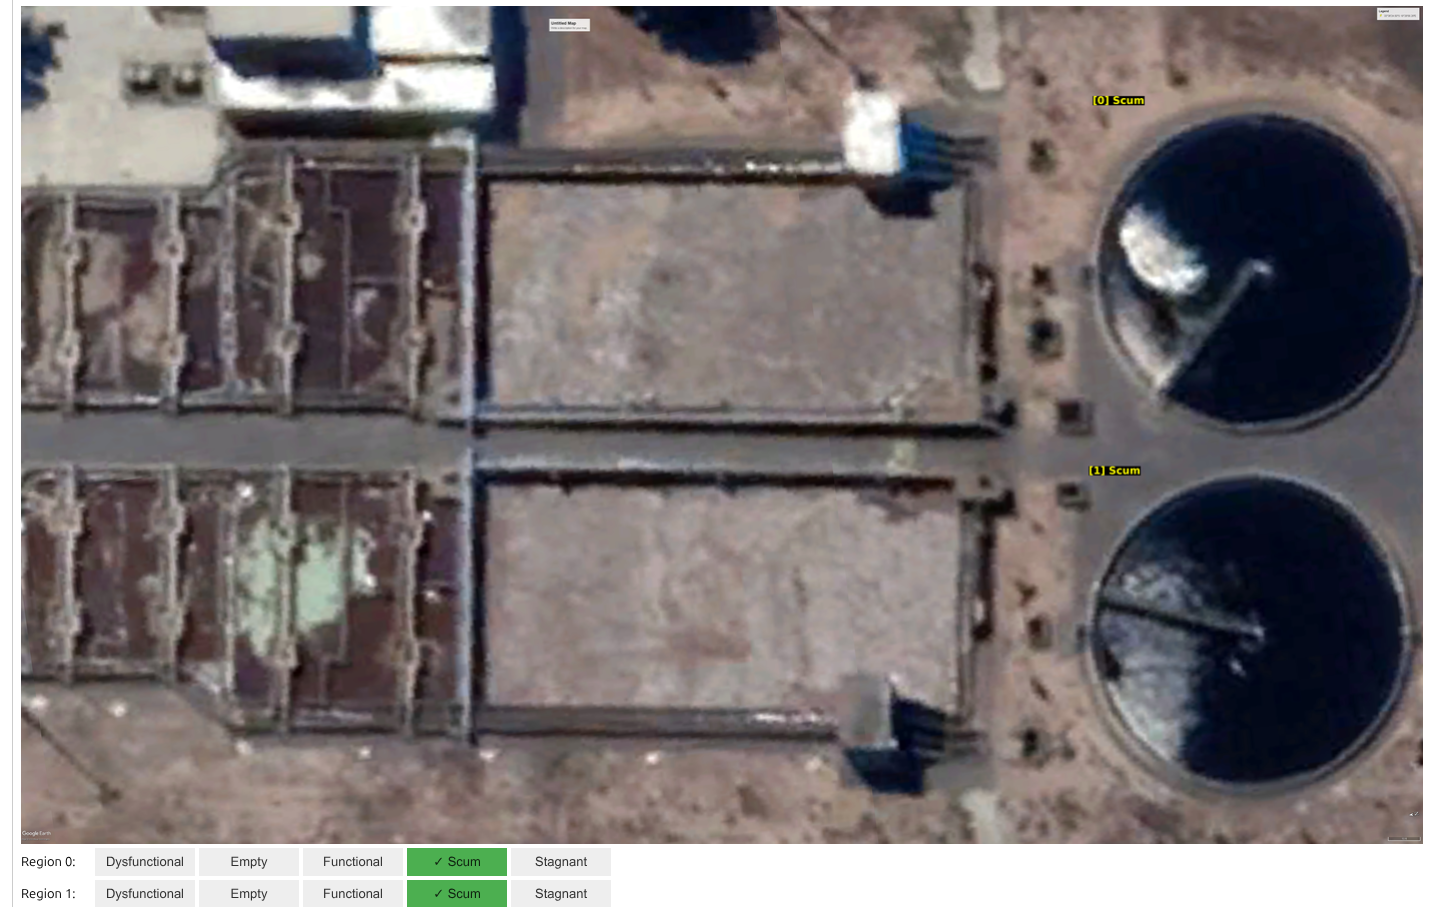
\includegraphics[width=0.55\textwidth]{figures/relabel_process_example.png}
\caption{The relabelling interface, showing the original label and the
per-class correction buttons.}
\label{fig:relabel_process_example}
\end{figure}

\section{Image Preprocessing and Normalisation}
\label{sec:appen_normalisation}

Every image passes through the same sequence of steps before it is given to a network. The steps are applied in the following order:

\begin{enumerate}
    \item \textbf{Letterbox resizing.} The image is scaled so that it fits the input size of the network ($224\times224$ pixels for the clarifiers and $112\times224$ pixels for the aerobic zones) without changing its aspect ratio. The remaining area is padded with zeros, with the image centred.
    \item \textbf{Augmentation.} For the training images only, random horizontal flips, random rotations of up to $15^\circ$, and random changes in brightness, contrast, saturation and hue are applied (Section~\ref{sec:exp_augmentation}). The development and test images are not augmented.
    \item \textbf{Scaling to $[0, 1]$.} The 8-bit pixel values, which lie in the range 0--255, are divided by 255 so that every value lies in the range $[0, 1]$.
    \item \textbf{Per-channel standardisation.} Each of the red, green and blue channels is standardised separately as
    \begin{equation}
        x' = \frac{x - \mu_c}{\sigma_c},
    \end{equation}
    where $x$ is the scaled pixel value, and $\mu_c$ and $\sigma_c$ are the ImageNet mean and standard deviation of channel $c$, given in Table~\ref{tab:imagenet_norm}.
\end{enumerate}

\begin{table}[htbp]
\centering
\caption{The per-channel ImageNet mean and standard deviation used to normalise the images.}
\label{tab:imagenet_norm}
\begin{tabular}{lccc}
\toprule
 & \textbf{Red} & \textbf{Green} & \textbf{Blue} \\
\midrule
Mean $\mu_c$ & 0.485 & 0.456 & 0.406 \\
Standard deviation $\sigma_c$ & 0.229 & 0.224 & 0.225 \\
\bottomrule
\end{tabular}
\end{table}

After standardisation, the values of each channel lie approximately in the range $[-2.1, 2.6]$ and are centred near zero. The ImageNet statistics are used rather than statistics computed from the WWTW dataset, since the pretrained backbones were trained on inputs normalised with these values. The same normalisation is applied to the images used for the Grad-CAM analysis.
